\documentclass[a4paper,10pt]{book}
\usepackage[pdftex]{graphicx}
\usepackage{epstopdf}
\usepackage{subfigure}
\usepackage{amsmath,amsthm}
\usepackage{tikz}
\usepackage{circuitikz}
\usetikzlibrary{babel}
\usetikzlibrary{shapes, arrows, patterns, angles, quotes}
\textwidth= 15cm
\evensidemargin=0cm
\usepackage[spanish]{babel}
\usepackage[utf8]{inputenc}
\usepackage{textcomp}
\usepackage{amstext}
\usepackage{amsfonts}
\usepackage{amssymb}
\usepackage{comment}
\usepackage[hyperindex=true,breaklinks=true,colorlinks=true,linkcolor=blue]{hyperref}
\renewcommand{\tablename}{Tabla}
\renewcommand{\listtablename}{\'Indice de Tablas}

\usepackage{listings}
\usepackage{color} %red, green, blue, yellow, cyan, magenta, black, white
\definecolor{mygreen}{RGB}{28,172,0} % color values Red, Green, Blue
\definecolor{mylilas}{RGB}{170,55,241}

\usepackage{multirow}
\usepackage{makeidx}

%\usepackage{draftwatermark}
%\SetWatermarkText{Borrador,juan.jimenez@fis.ucm.es}
%\SetWatermarkScale{2}

% Atajos para el tikz
\tikzstyle{block} = [draw, rectangle, minimum width=6em]
\tikzstyle{sum} = [draw, fill=blue!20, circle, node distance=1cm]
\tikzstyle{input} = [coordinate]
\tikzstyle{output} = [coordinate]
\tikzstyle{pinstyle} = [pin edge={to-,thin,black}]

% Entornos para los "teoremas"
\newtheorem{algo}{Algoritmo}[section]
\newtheorem{theorem}{Teorema}[section]
\newtheorem{problem}{Problema}[section]
\newtheorem{corollary}{Corolario}[section]
\newtheorem{lemmas}{Lema}[section]
\newcommand*{\lema}{Lema}
\newenvironment{lemma}[1][\lema]{\begin{lemmas}[#1]\renewcommand*{\qedsymbol}{\(\Diamond\)}}{\end{lemmas}}

\theoremstyle{definition}
%\newtheorem{definition}{Definición}[section]
\newtheorem{definitions}{Definición}[section]
\newcommand*{\definicion}{Definición}
\newenvironment{definition}[1][\definicion]{\begin{definitions}[#1]\renewcommand*{\qedsymbol}{\(\bigtriangledown\)}}{\end{definitions}}

\newtheorem{examples}{Ejemplo}[section]
\newcommand*{\ejemplo}{Ejemplo}
\newenvironment{example}[1][\ejemplo]{\begin{examples}[#1]\renewcommand*{\qedsymbol}{\(\maltese\)}}{\end{examples}}
%\renewcommand{\qedsymbol}{\maltese}

\theoremstyle{remark}
\newtheorem{remark}{Atención}[section]

\graphicspath{{./figuras/}}
\makeindex
\begin{document}
\title{
\begin{flushleft}

\includegraphics[width=2.5cm]{ucm2.eps}
Universidad Complutense de Madrid\\
---------------------------------------------------------------------\
\end{flushleft}
Manual de Paparazzi}
\author{ UCM237}

\maketitle\
\
\vspace*{\fill}

\includegraphics[scale=1]{by-sa.eps}\\
El contenido de estos apuntes est\'e1 bajo licencia Creative Commons Atribution-ShareAlike 4.0\\
\href{http://creativecommons.org/licenses/by-sa/4.0/}{http://creativecommons.org/licenses/by-sa/4.0/}\\
\copyright Juan Jim\'enez

\bigskip
\tableofcontents
\listoffigures
%\listoftables
%\section*{Matlab Code}
\lstset{language=Matlab,%
    %basicstyle=\color{red},
    breaklines=true,%
    morekeywords={matlab2tikz},
    keywordstyle=\color{blue},%
    morekeywords=[2]{1}, keywordstyle=[2]{\color{black}},
    identifierstyle=\color{black},%
    stringstyle=\color{mylilas},
    commentstyle=\color{mygreen},%
    showstringspaces=false,%without this there will be a symbol in the places where there is a space
    numbers=left,%
    numberstyle={\tiny \color{black}},% size of the numbers
    numbersep=9pt, % this defines how far the numbers are from the text
    emph=[1]{for,end,break},emphstyle=[1]\color{red}, %some words to emphasise
    %emph=[2]{word1,word2}, emphstyle=[2]{style},    
}

Esto es un simple guía burros para paparazzi, dado que entender lo que dice es complicadillo.
En principio, podemos dividirlo en capítulos, y emplear para cada uno un archivo nuevo.

De todos modos, lo importante es ir escribiendo y luego vemos como organizarlo. \\

Antes de comenzar, indicar que a lo largo de todo este documento vamos a trabajar con Linux, más concretamente con el sistema operativo Ubuntu en su versión 20.04. Este es el único entorno que va a soportar PaparazziUAV.\\

\noindent El equipo que desarrolla PaparazziUAV cuenta con una wiki muy detallada que puede llegar a ser muy útil para incorporarse al entorno: \url{https://wiki.paparazziuav.org/wiki}. Para instalar PaparazziUAV recomendamos al usuario seguir directamente la entrada \textit{installation} (\url{https://wiki.paparazziuav.org/wiki/Installation}) y leer el \textit{README.md} principal del proyecto (\url{https://github.com/UCM-237/paparazzi}). \\
\chapter{Paparazzi Center}

% TODO: ¿Sección de instalación?

\noindent Una vez realizada la instalación, podremos ejecutar el binario precompilado \textit{paparazzi} que se encuentra en la carpeta raíz de Paparazzi. Entonces se inicializará todo el ecosistema y se ejecutará Paparazzi Center, el panel de control principal de PaparazziUAV [Figura \ref{fig:cap1_interfaz}]. En él nos encontraremos inicialmente con un proyecto (A/C) ejemplo. Dentro de cada proyecto podremos introducir varios \textbf{archivos de configuración .xml} (en el capítulo sobre el directorio \textit{conf} explicaremos más detalladamente para qué sirve cada uno):

\begin{enumerate}
    \item \textbf{Airframe}: va a contener toda la información sobre el hardware y firmware de nuestro vehículo. \url{https://wiki.paparazziuav.org/wiki/Airframe_Configuration}.
    
    \item \textbf{Flight Plan}: definirá la geolocalización, los bloques y los waypoints que aparecerán en el modo navegación.
    
    \item \textbf{Radio}: ajustará las ganancias y la funcionalidad de los canales del radio control. Paparazzi ya trae la configuración de varios modelos, si nuestro controlador no se encuentra entre ellos deberemos de generar su .xml teniendo en cuenta sus especificaciones.
    
    \item \textbf{Telemetry}: definirá los distintos modos de telemetría del vehículo y los mensajes que se enviarán en cada uno de ellos. 
    
\end{enumerate}

\begin{figure}[h!]
    \centering
    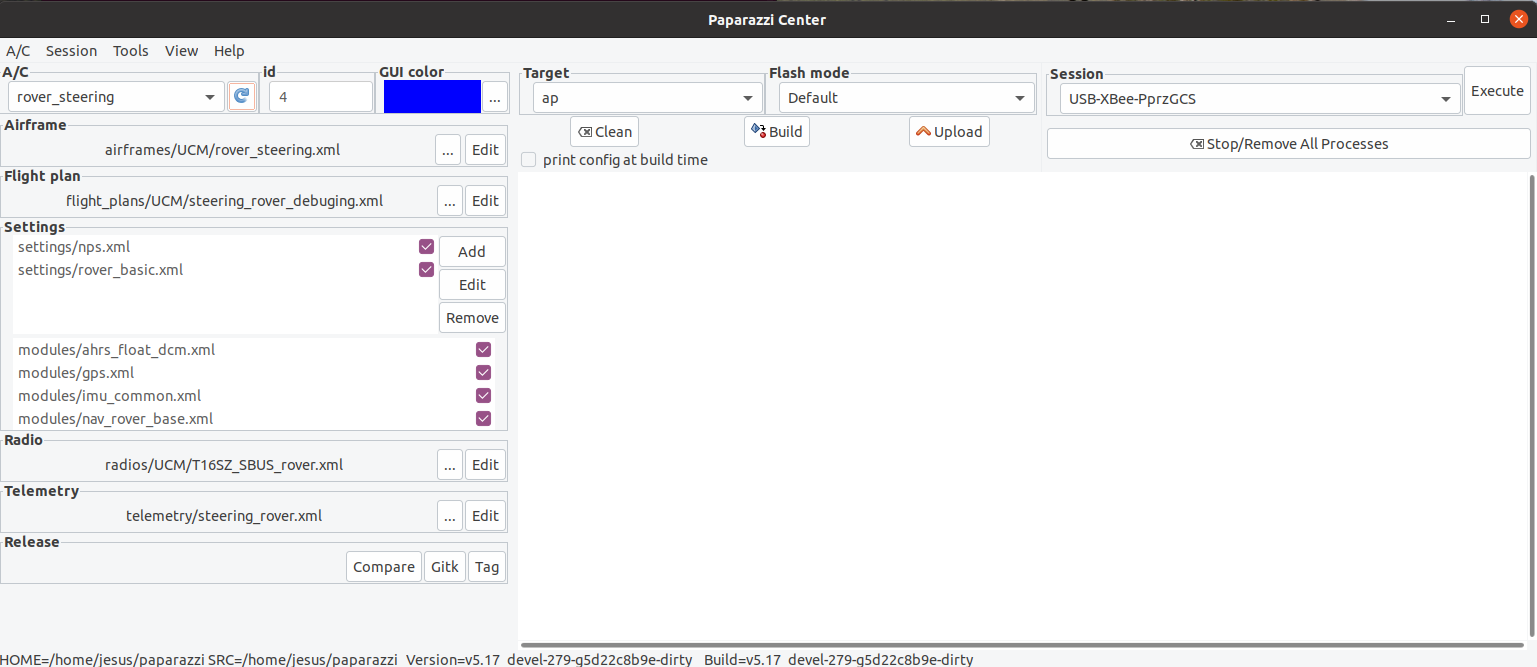
\includegraphics[width=0.8\textwidth]{./figuras/cap1_interfaz.png}
    \caption{Interfaz de Paparazzi Center, el panel de control principal de PaparazziUAV.} \label{fig:cap1_interfaz}
\end{figure}

\newpage

Para compilar ... \\

Herramientas y sesiones ... \\


\chapter{Ground control station} 
\chapter{El directorio conf}
\chapter{El directorio sw}
\chapter{Un ejemplo completo: Rover Steering}
\printindex
\end{document} 
